\section*{\centering {Supplementary Materials}} \label{sec:supplement}

\section{Some Examples}

Here are the supplementary materials. This is a dynamic input: $0.889~[0.880, 0.891]%$.

\subsection{Example Figure}

\begin{figure}[h!]
	\centering
	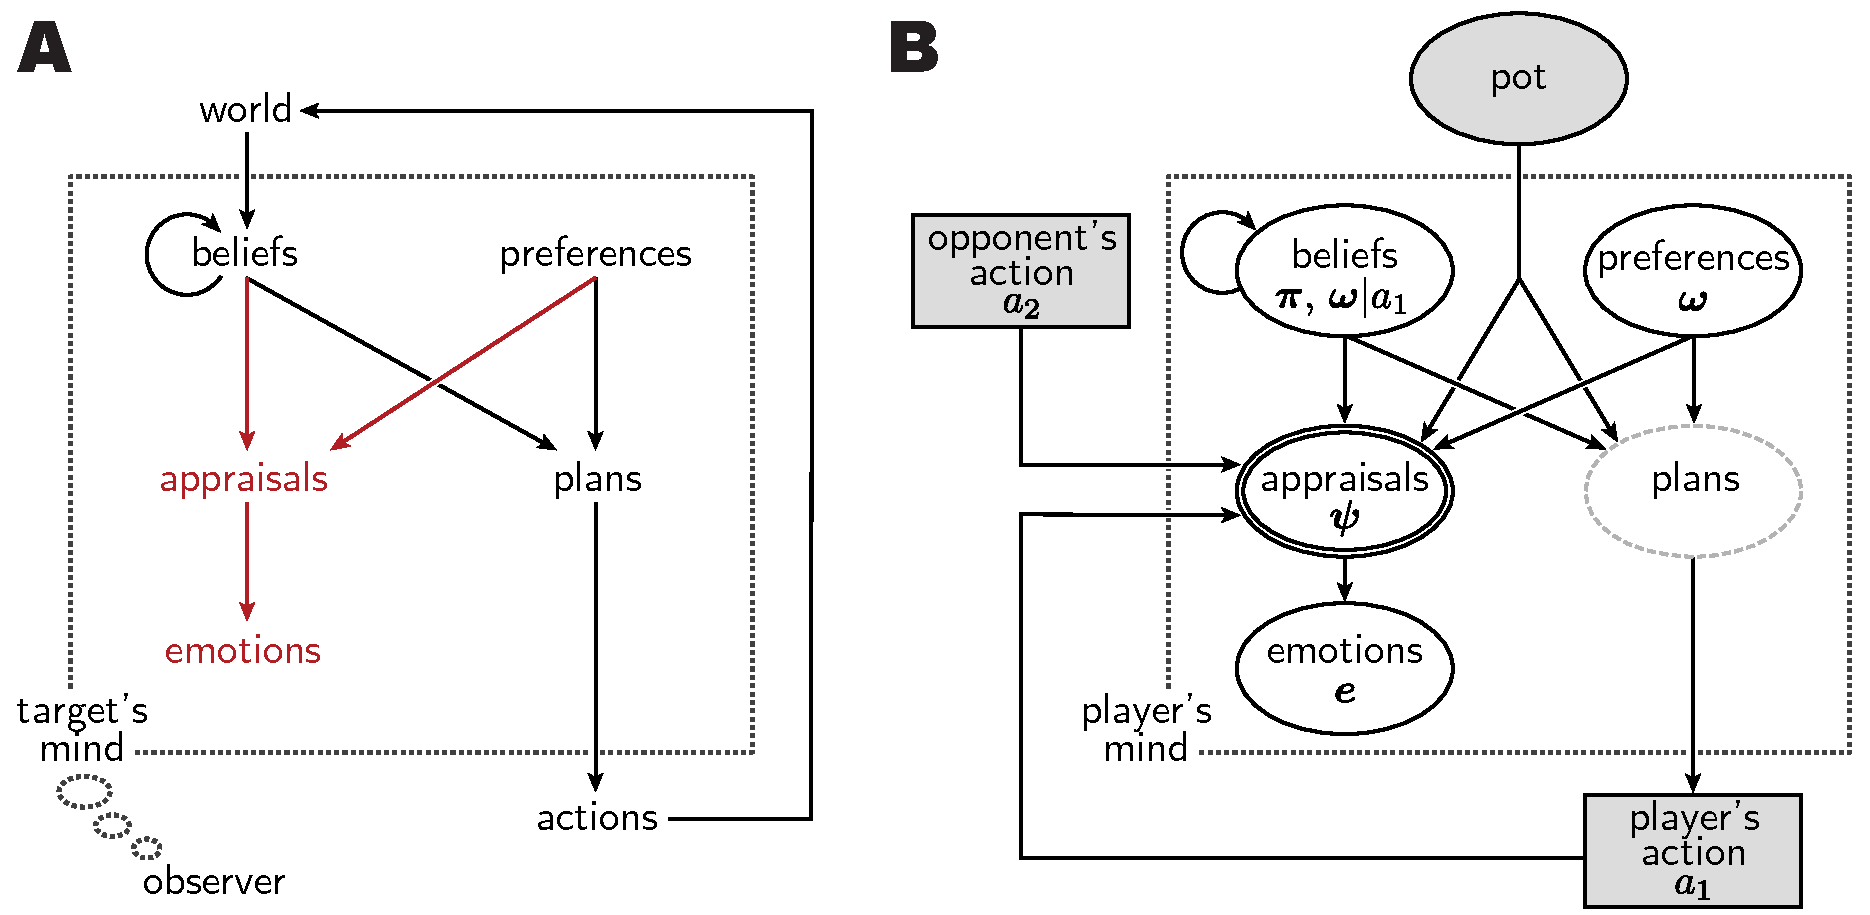
\includegraphics[width=1\textwidth,keepaspectratio]{figs/model_diagram.pdf}
	\caption{\textbf{Emotion prediction as inference over an intuitive Theory of Mind.} 
	Hypotheses about how human observers reason about others' emotions can be formalized as probabilistic generative models.
	}
	\label{fig:supp:dag}
\end{figure}

\subsection{Example Table}

\begin{table}[h!]
\begin{center} 
\caption{Sample table title.} 
\label{sample-table} 
\vskip 0.12in
\begin{tabular}{ll} 
\hline
Error type    &  Example \\
\hline
Take smaller        &   63 - 44 = 21 \\
Always borrow~~~~   &   96 - 42 = 34 \\
0 - N = N           &   70 - 47 = 37 \\
0 - N = 0           &   70 - 47 = 30 \\
\hline
\end{tabular} 
\end{center} 
\end{table}
